\documentclass[12pt,a4paper]{amsart}
% ukazi za delo s slovenscino -- izberi kodiranje, ki ti ustreza
\usepackage[slovene]{babel}
%\usepackage[cp1250]{inputenc}
\usepackage[T1]{fontenc}
\usepackage[utf8]{inputenc}
\usepackage{amsmath,amssymb,amsfonts}
\usepackage{url}
\usepackage{graphicx}
%\usepackage[demo]{graphicx}
%\usepackage[normalem]{ulem}
\usepackage[dvipsnames,usenames]{color}
\usepackage{hyperref}
\usepackage{float}
\usepackage{adjustbox}

\usepackage{xcolor}
\hypersetup{
    colorlinks,
    linkcolor={red!50!black},
    citecolor={blue!50!black},
    urlcolor={blue!80!black}
}

% ne spreminjaj podatkov, ki vplivajo na obliko strani
\textwidth 15cm
\textheight 24cm
\oddsidemargin.5cm
\evensidemargin.5cm
\topmargin-5mm
\addtolength{\footskip}{10pt}
\pagestyle{plain}
\overfullrule=15pt % oznaci predlogo vrstico
\setlength{\parskip}{1.3ex}

% ukazi za matematicna okolja
\theoremstyle{definition} % tekst napisan pokoncno
\newtheorem{definicija}{Definicija}[section]
\newtheorem{primer}[definicija]{Primer}
\newtheorem{opomba}[definicija]{Opomba}

\renewcommand\endprimer{\hfill$\diamondsuit$}


\theoremstyle{plain} % tekst napisan posevno
\newtheorem{lema}[definicija]{Lema}
\newtheorem{izrek}[definicija]{Izrek}
\newtheorem{trditev}[definicija]{Trditev}
\newtheorem{posledica}[definicija]{Posledica}


% za stevilske mnozice uporabi naslednje simbole
\newcommand{\N}{\mathbb N}
\newcommand{\C}{\mathbb C}
\newcommand{\Q}{\mathbb Q}

\newcommand{\X}{\mathcal X}
\newcommand{\Y}{\mathcal Y}
\newcommand{\Z}{\mathcal Z}
\newcommand{\B}{\mathcal B}
\newcommand{\R}{\mathcal R}

% ukaz za slovarsko geslo
\newlength{\odstavek}
\setlength{\odstavek}{\parindent}
\newcommand{\geslo}[2]{\noindent\textbf{#1}\hspace*{3mm}\hangindent=\parindent\hangafter=1 #2}

% naslednje ukaze ustrezno popravi
\newcommand{\program}{Finančna matematika} % ime studijskega programa: Matematika/Finan"cna matematika
\newcommand{\imeavtorja}{Luka Lodrant} % ime avtorja
\newcommand{\imementorja}{Janoš Vidali} % akademski naziv in ime mentorja
\newcommand{\naslovdela}{Razbitje grafa na dva disjunktna liha podgrafa}
\newcommand{\letnica}{2019} %letnica


% vstavi svoje definicije ...

\DeclareMathOperator{\GF}{GF}
\DeclareMathOperator{\NGG}{N_G}


\begin{document}

% od tod do povzetka ne spreminjaj nicesar
\thispagestyle{empty}
\noindent{\large
UNIVERZA V LJUBLJANI\\[1mm]
FAKULTETA ZA MATEMATIKO IN FIZIKO\\[5mm]
\program\ -- 1.~stopnja}
\vfill

\begin{center}{\large
\imeavtorja\\[2mm]
{\bf \naslovdela}\\[10mm]
Projekt v povezavi z OR\\[1cm]}

\end{center}
\vfill

\noindent{\large
Ljubljana, \letnica}
\pagebreak

\thispagestyle{empty}
\hypersetup{linkcolor = black}
\tableofcontents
\pagebreak

\section{Navodilo}

In the paper
https://arxiv.org/abs/1802.07991
the authors gave a characterization when a graph can be decomposed into two disjoint odd subgraphs.
Their result, based on the Gaussian elimination method, implies a polynomial time algorithm to verify this kind od decomposability.
Implement this algorithm; then for small values of n, verify the percentage of graphs on n vertices that can be decomposed in the prescribed way.
Similarly, you can also consider other classes of graphs, say small bipartite graphs, trees, \ldots


\section{Uvod}

Osnovni predmet obravnave tega dela bodo \emph{multigrafi}, ki lahko vzporedne povezave, nimajo pa zank. Grafu brez podvojenih povezav in zank rečemo \emph{enostaven graf}.
Naj bo $G=(V(G),  E(G))$ multigraf. Z $OddV(G)$ bomo označili množico oglišč z lihimi stopnjami, z $EvenV(G)$ pa množico oglišč s sodimi stopnjami.
Lih (oz. sod) podgraf grafa $G$ je podgraf, katerega vsa oglišča so lihe (oz. sode) stopnje.

Naš cilj je, da ugotovimo, kdaj je možno graf razbiti na 2 podgrafa lihe stopnje in za to implementirati polinomski algoritem.
Z uporabo tega algoritma pa bomo v drugem delu analizirali kakšen delež posebnih kategorij grafov je možno na tak način razbiti.

Projekt bomo implementirali v programskem jeziku \emph{Python 3}, veliko pa bomo uporabljali knjižnico \emph{networkx} za delo z grafi.

\section{Matematična podlaga}

Kot prej, naj bo $G$ multigraf z oglišči $V(G)$ in povezavami $E(G)$. Z $EvenV(G)$ bomo označili oglišča sode stopnje, z $OddV(G)$ pa oglišča lihe stopnje.
Za množico oglišč $U$ grafa $G$, naj bo $\langle U \rangle_G$ podgraf induciran na teh ogliščih. Red grafa označimo z $|G|$ in pomeni število oglišč v grafu.

\begin{definicija}
Graf $G$ je \emph{lih}, če je stopnja vsakega oglišča grafa liha.
\end{definicija}

\begin{definicija}
\emph{Liho razbitje grafa} $G$ dobimo tako, da je tako razbitje povezav grafa na 2 disjunktni množici $U$ in $V$, da vsaka inducira lih podgraf.
\end{definicija}

\begin{definicija}
Imamo graf $G = (V, E)$ in množico oglišč $T \subseteq V$. \emph{T-join} je taka podmnožica povezav $J \subseteq E$,
da imajo v grafu $(V, J)$ vsa oglišča iz $T$ liho stopnjo.
\end{definicija}

Za graf $G$ nas torej zanima ali liho razbitje obstaja in kakšno je.
Tu bomo opisali polinomski algoritem za ta izračun, dokaz in ideja tega algoritma pa sta na voljo v

Naj bo $\X$ množica povezanih komponent grafa $\langle OddV(G) \rangle_G$. Množico povezanih komponent grafa $\langle EvenV(G) \rangle_G$ razbijemo, množica $\Y$ naj vsebuje komponente lihega reda,
$\Z$ pa sodega.
Z $\NGG(U)$ označimo množici tistih $X_i \in \X$, ki so z $U$ povezani z lihim številom povezav.
Torej $\NGG(U)=\{\,X_i \in \X;\, e_G(U, X_i) \text{ je liho} \,\}$. Za vsak $X_i$ definiramo binarno spremenljivko $x_i$,
ki nam pove, ali bomo oglišča iz $X_i$ pobarvali z rdečo ($\R$) ali modro ($\B$).
V primeru $x=1$, bo $X_i \in \R$, v primeru $x=0$ pa $X_i \in \B$.

Sedaj sestavimo sistem linearnih enačb v polju $\GF(2)$:
\begin{align*}
\sum_{X_i \in \NGG(Y)} x_i &=1&   &\text{za}\ Y \in \Y\\
\sum_{X_i \in \NGG(Z)} x_i &=1&   &\text{za}\ Z \in \Z
\end{align*}

Ta sistem rešimo z uporabo primernih metod, v naši implementaciji smo uporabili klasično Gauss-Jordan eliminacijo.
Če sistem ni rešljiv, grafa $G$ ni možno razbiti na 2 liha podgrafa. Sedaj naj bo $x_1, \ldots, x_n$ ena izmed rešitev tega sistema.
Iz te rešitve sestavimo množici $\R$ in $\B$, nato pa vse povezave, ki mejijo na katerokoli oglišče iz unije $\R$ pobarvamo z rdečo.

Na tej točki imamo pobarvanih nekaj povezav, od katerih pa nobena ne povezuje množic $\R$ in $\B$, prav tako pa tudi nobena
ni del grafa $\langle EvenV(G) \rangle_G$. Z $T$ označimo množico vseh vozlišč grafa $G$, ki imajo sodo rdečo stopnjo (stopnjo, pri kateri gledamo le rdeče povezave).
Preostane nam še izračun \emph{T-join} na tem grafu.

Obravnavali bomo vsako povezano komponento posebej. Naj bodo $C_i$ povezane komponente grafa $G$ in definiramo še $T_i = C_i \cap T$.
Vsako $T_i$ razbijemo na pare $(u, v)$ (iz pravilnosti algoritma sledi, da je sodega reda) in najdemo preprosto pot med vozliščema $u$ in $v$.
Preprosta pot vsebuje vsako povezavo le enkrat, zaradi povezanosti mora obstajati.
Nato preštejemo, kolikokrat je bila vsaka povezava uporabljena v teh preprostih poteh. V naš \emph{T-join} spadajo tiste, ki so bile uporabljene liho krat.

Sedaj smo z našim algoritmom zaključili, vse povezave iz izračunanega \emph{T-joina} pobarvamo z rdečo,
z modro pa pobarvamo vse še nepobarvane povezave. Če je algoritem uspel (linearni sistem je bil rešljiv), modro in rdeče
pobarvane povezave inducirajo dva liha podgrafa grafa $G$. %  slika uspeha


\section{Implementacija algoritma}
Kot že povedano smo se implementacije lotili v programskem jeziku \emph{Python 3}, za delo z grafi smo se odločili za uporabo knjižnice \emph{networkx}.
Algoritem je implementiran v datotek \emph{decomposition/decomposition.py}.

Pri reševanju linearnega sistema v $\GF(2)$ smo si pomagali z \emph{Matrix} razredom~\cite{field}.

Ko smo enkrat razumeli, kako prej opisan algoritem deluje, njegova implementacija ni bila posebno zahtevna, vse je bolje opisano v komentarjih poleg kode.
Paziti je bilo potrebno na par posebnih primerov, kot npr. razbitje že lihega grafa, pri katerem linearni sistem ne obstaja.

\section{Analiza posebnih grafov}

\subsection{Mali grafi}
\emph{decomposition/small\_graphs.py}

Prva stvar, ki nas je zanimala, je bila kolikšen delež grafov na malem številu oglišč je možno razbiti na dva liha grafa.
Grafe smo zgenerirali tako, da smo za vsak $n$ sestavili množico vseh možnih povezav v grafu, potem pa sestavili njeno potenčno množico.
Iz te skupine grafov smo nato še odstranili vse grafe z izoliranimi vozlišči, saj so to efektivno grafi na manj vozliščih.
Nato smo vsak tako dobljen graf poskusili razbiti in le prešteli, za koliko grafov je bilo to možno.

Do $n=7$ je tak princip deloval, nato pa smo pri $n=8$ prišli do težave, saj na toliko vozliščih obstaja kar $268435456 \approx 2.6 * 10^8$ grafov.
Z osnovnim algoritmom bi tako potrebovali približno $110h \approx 4,5 dneva$, kar pa nismo želeli. Algoritem smo najprej malo optimizirali, namesto sesnamov smo
na primernih mestih uporabili sete oz. generatorje, in na začetku preverili ali ima graf kakšno izolirano oglišče, saj takšnega grafa ni mogoče razbiti.

To ni bilo dovolj, ocenjeni čas je zmanjšalo le na približno $70h$. Sedaj bi lahko poskusili algoritem še izboljšati z uporabo nižjenivojskega jezika in bolj
primernih podatkovnih struktur, kar pa bi nam lahko vzelo precej več dela. Namesto tega, smo se odločili, da bomo le uporabili malo več procesorske moči. Primerno
smo razbili našo testno množico in paralelizirali razbitja z uporabo knjižnice \emph{joblib}.
Tako smo na enem samem osemjedrnem računalniku s 14 nitmi prišli do tega, da je izračun trajal "le" $4.5h$.

\noindent Rezultate testov predstavimo v tabeli in pa v grafih:

\begin{adjustbox}{width={\textwidth},totalheight={\textheight},keepaspectratio}%
\begin{tabular}{|l|l|l|l|l|}
\hline
\textbf{število vozlišč} & \textbf{število grafov} & \textbf{število uspešnih} & \textbf{uspešnost} & \textbf{čas izvajanja} \\ \hline
3           & 8            & 3                & 37.50 \%     & 0.82 s         \\ \hline
4           & 64           & 35               & 54.68 \%     & 0.49 s         \\ \hline
5           & 1024         & 345              & 33.69 \%     & 0.66 s         \\ \hline
6           & 32768        & 19894            & 60.71 \%     & 3.36 s         \\ \hline
7           & 2097152      & 638967           & 30.47 \%     & 144 s          \\ \hline
8           & 186344860    & 268435456        & 69.42 \%     & 50278 s        \\ \hline
\end{tabular}
\end{adjustbox}

\begin{figure*}[h]
\centering
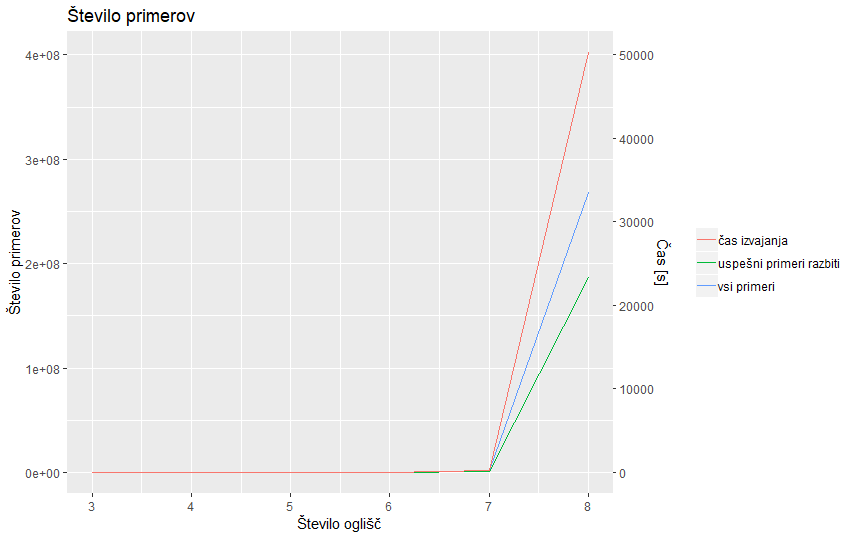
\includegraphics[width=1\textwidth]{images/sm_graph_cases}
\end{figure*}

Prvi graf nam za občutek prikaže kako hitra je rast števila grafov, zanima pa nas predvsem drugi.

\begin{figure*}[h]
\centering
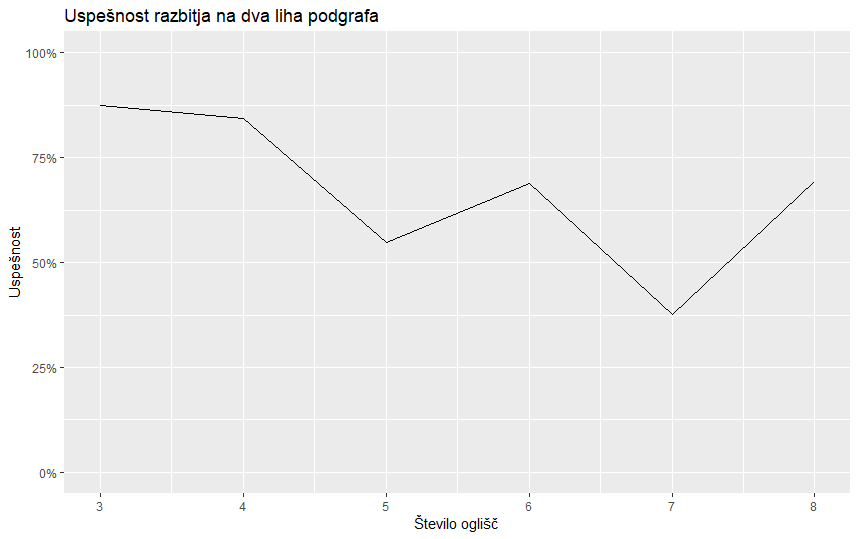
\includegraphics[width=1\textwidth]{images/sm_graph_success}
\end{figure*}


Tukaj prvič vidimo nihanje uspešnosti med lihimi in sodimi števili vozlišč. Na lihih je uspešnost razbitja
manjša kot na sodih. Ta rezultat bomo kasneje videli tudi v drugih primerih grafov.
Jasnih trendov na tem grafu ne moremo opaziti, saj imamo premalo podatkov.
Tisti pri $n=3$ in $n=4$ zaradi malega števila grafov samih niso realen pokazatelj trenda.

\subsection{Izomorfni razredi grafov}
\emph{decomposition/small\_graphs\_isomorphic.py}
%http://users.cecs.anu.edu.au/~bdm/data/graphs.html

Tako opazimo, da z analizo vseh možnih grafov ne bomo prišli daleč, saj njihovo število prehitro raste.
Malo dlje lahko pridemo tako, da se omejimo le na izomorfne razrede grafov.
Teh ne bomo generirali samo, temveč smo jih prenesli iz \cite{isomorph} v obliki \emph{graph6}.

Rezultate spet predstavimo z isto tabelo in grafi.

\begin{adjustbox}{width={\textwidth},totalheight={\textheight},keepaspectratio}%
\begin{tabular}{|l|l|l|l|l|}
\hline
\textbf{število vozlišč} & \textbf{število grafov} & \textbf{število uspešnih} & \textbf{uspešnost} & \textbf{čas izvajanja} \\ \hline
2    & 2            & 2         & 100.00 \%   & 0.61 s     \\ \hline
3    & 4            & 3         & 75.00 \%    & 0.39 s     \\ \hline
4    & 11           & 9         & 81.81 \%    & 0.38 s     \\ \hline
5    & 34           & 19        & 55.88 \%    & 0.36 s     \\ \hline
6    & 156          & 109       & 69.87 \%    & 0.09 s     \\ \hline
7    & 1044         & 428       & 41.00 \%    & 0.62 s     \\ \hline
8    & 12346        & 8465      & 68.56 \%    & 7.66 s     \\ \hline
9    & 274668       & 82138     & 29.90 \%    & 50.1 s     \\ \hline
10   & 12005168     & 8910781   & 74.22 \%    & 3043 s     \\ \hline
\end{tabular}
\end{adjustbox}

\begin{figure*}[h]
\centering
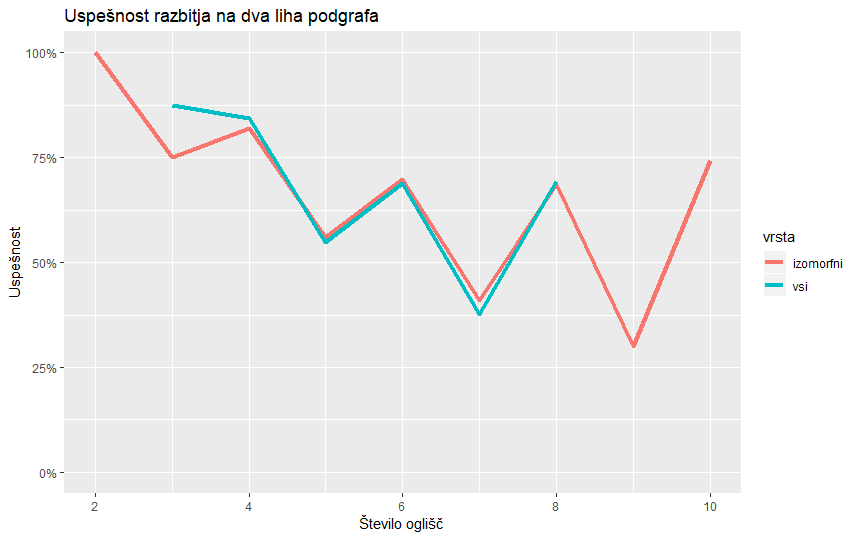
\includegraphics[width=1\textwidth]{images/success_isomorphic.png}
\end{figure*}

Na graf smo dodali tudi uspešnost na vseh in vidimo, da se skoraj ujemata.
Bolje lahko prepoznamo tudi vzorec lihih in sodih, kjer je pri lihin $n$ uspešnost nižja
kot pri sodih. Opazimo lahko tudi, da za lihe $n$ uspešnost pada, medtem ko za sode počasi raste, vendar
ne moremo trditi, da je to pravilo, saj je podatkov premalo.
\pagebreak

\subsection{Vpliv števila povezav}
\emph{decomposition/random\_graphs.py}

Zanima nas, kako število povezav vpliva na razcepnost grafov pri istem številu oglišč. Za ta namen pri konstatnem številu
oglišč $n$ generirali po 10000 naključnih grafov z $m$ povezavami za vsak možen $m$. To bomo storili z uporabo funkcije \texttt{nx.gnm\_random\_graph(n, m)},
ki nam z enako verjetnostjo vrne vsak graf z $n$ oglišči in $m$ povezavami. To bomo storili tudi za več razliščnih $n$ in
poskusili ugotoviti, ali med vsemi temi parametri obstaja kakšna povezava.

Grafe bomo generirali naključno, saj nas ta vpliv zanima za velike $n$ za katere ne moremo preizkusiti vseh. Izbrali smo si
analizo $n$ od $20$ do $23$.
Tabela nam v tem primeru ne pomaga, zato si le izrišemo graf uspešnosti v odvisnosti od števila povezav.

\begin{figure*}[h]
\centering
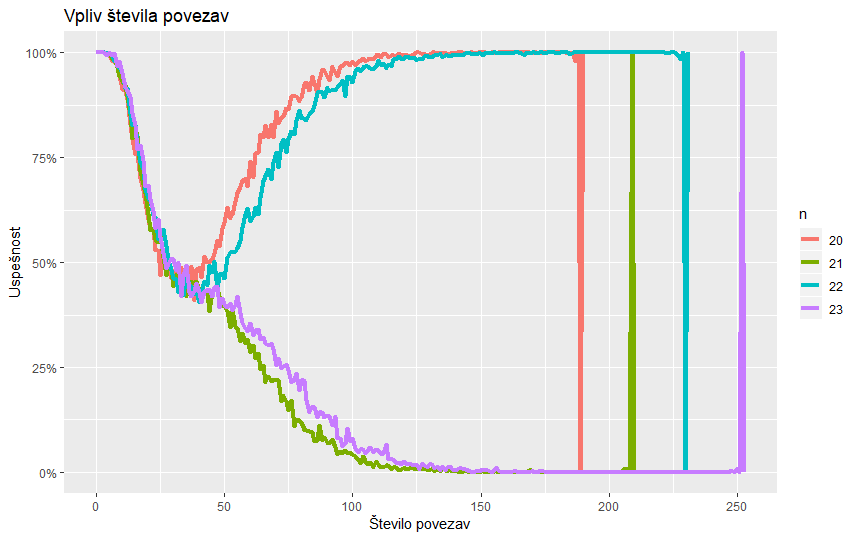
\includegraphics[width=1\textwidth]{images/random_graphs.png}
\end{figure*}

Spet lahko ločimo sode od lihih primerov. Na lihem številu vozlišč verjetnost s številom povezav
pada, medtem ko za sode velja, da so grafi z malim in tisti z velikim številom povezav so večinoma razcepni, za tiste vmes pa je verjetnost,
da so razcepni nižja. Pri grafu z vsemi povezavami oz. tistemu z eno manj vidimo, da razcepnost skoči,
to pa le zato, ker tak graf obstaja le en, in je zato lahko verjetnost le $0$ oz. $1$.

\pagebreak

\subsection{Čas delovanja}
\emph{decomposition/timedifficulty.py}

Za konec lahko preverimo še, kako z rastjo števila oglišč raste čas izvajanja algoritma.
Za ta namen bomo grafe spet generirali naključno, ampak drugače kot prej. Namesto fiksnega števila
povezav, bomo za vsako povezavo rekli, da jo z verjetnostjo $0.7$ dodamo v graf.
Nato smo za vsak deseti $n$ poskusili razbiti $100$ takšnih grafov in izračunali povprečen čas izvajanja za en primer.

\begin{figure*}[h]
\centering
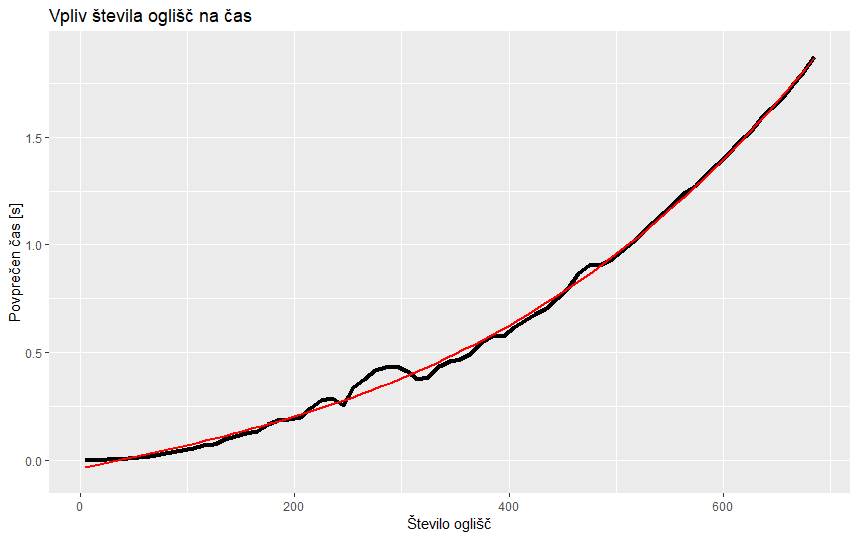
\includegraphics[width=1\textwidth]{images/timed.png}
\end{figure*}


Čase izvajanja prikažemo na grafu in vidimo, da se polinomska krivulja tretje stopnje zelo prilega,
kar tudi empirično potrjuje teoretično časovno zahtevnost. Odstopanja nastajajo zaradi majhnega števila
naključnih primerov. Če bi to število dvignili, je linija bolj gladka, ampak za izračun porabimo preveč časa.
Za naše potrebe je 100 primerov vsake velikosti povsem dovolj.


\section{Zaključek}

\begin{thebibliography}{9}

\bibitem{base} M. Kano, G. Y. Katona, K. Varga (2018). Decomposition of a graph into two disjoint. Pridobljeno iz spletne strani: \url{https://arxiv.org/abs/1802.07991}.
\bibitem{field} Project Nayuki (2017). Gauss-Jordan elimination over any field. Pridobljeno iz spletne strani: \url{https://www.nayuki.io/page/gauss-jordan-elimination-over-any-field}.
\bibitem{tjoin} C. Chekuri, B. Raichel (2010). Combinatorial Optimization (Lecture). Pridobljeno iz spletne strani: \url{https://courses.engr.illinois.edu/cs598csc/sp2010/Lectures/Lecture13.pdf}.
\bibitem{isomorph} B. McKay. Graphs (spletni vir). Pridobljeno iz spletne strani: \url{http://users.cecs.anu.edu.au/~bdm/data/graphs.html}.


\end{thebibliography}

\end{document}